\chapter{Variables and types}

This chapter is about storing values in computer memory and doing simple arithmetic.
More importantly, it's about how to compose statements using basic building blocks such as variables, keywords, operators, and expressions.


\section{Variables}

\index{variable}
\index{value}

One of the most powerful features of a programming language is the ability to define and manipulate {\bf variables}.
A variable is a named location of computer memory that stores a single {\bf value}.
Values may be numbers, text, images, sounds, and other types of data.
%They can be printed, and as we'll see later, operated on.
To store a value in memory, you first have to create a variable.
%Since the values we want to store are text, we declare that the new variable is a string:

\begin{code}
    String message;
\end{code}

\index{declaration}
\index{statement!declaration}
\index{type!int}
\index{type!char}
\index{type!String}

This statement is a {\bf declaration}, because it declares that the variable named \java{message} has the type \java{String}.
Each variable has a {\bf type} that determines what kind of values it can store.
For example, the \java{int} type can store integers, and the \java{char} type can store characters.

Some types begin with a capital letter and some with lower-case.
We will learn the significance of this distinction later, but for now you should take care to get it right.
There is no such type as \java{Int} or \java{string}, and the compiler will complain if you try to make one up.

To declare an integer variable, the syntax is:

\begin{code}
    int value;
\end{code}

Note that \java{value} is an arbitrary name for the variable.
In general, you will want to make up variable names that indicate what you plan to do with the variable.
For example, if you saw these variable declarations, you could probably guess what values would be stored in them:

\begin{code}
    String firstName;
    String lastName;
    int hour, minute;
\end{code}

This example also demonstrates the syntax for declaring multiple variables with the same type: \java{hour} and \java{second} are both integers.
Note that each declaration statement ends with a semicolon.


\section{Keywords}
\index{keyword}

You can make up just about any name you want for a variable.
But there are certain words that are reserved in Java, because they are used by the compiler to parse the structure of the program.
These words, called {\bf keywords}, include \java{public}, \java{class}, \java{static}, \java{void}, \java{int}, and many more.
Search the Internet for ``Java keywords'' to see the complete list.

%The complete list is available at \url{https://docs.oracle.com/javase/tutorial/}.
%This site, provided by Oracle, includes Java documentation I refer to throughout the book.

Rather than memorize the keywords, you should take advantage of the syntax highlighting provided in many development environments (including DrJava).
As you type, the tokens in your program will appear in different colors.
For example, keywords might be blue, strings red, comments green, and other code black.
If you type a variable name and it turns blue, watch out!


\section{Assignment}

\index{assignment}
\index{statement!assignment}

Now that we have created variables, we want to store values.
We do that with an {\bf assignment} statement.

\begin{code}
    message = "Hello!";  // give message the value "Hello!"
    hour = 11;           // assign the value 11 to hour
    minute = 59;         // set minute to 59
\end{code}

This example shows three assignments, and the comments show three different ways people sometimes talk about assignment statements.
The vocabulary can be confusing here, but the idea is straightforward:

\begin{itemize}
\item When you declare a variable, you create a named storage location.
\item When you make an assignment to a variable, you give it a value.
\end{itemize}

A common way to represent variables on paper is to draw a box with the name of the variable on the outside and the value of the variable on the inside.
The diagram below shows the effect of the three assignment statements:

\begin{center}
\begin{tabular}{rl}
message & \framebox[2cm]{Hello!} \\
   hour & \framebox[1cm]{11} \\
 minute & \framebox[1cm]{59} \\
\end{tabular}
\end{center}

As a general rule, a variable has to have the same type as the value you assign to it.
You cannot store a \java{String} in \java{minute} or an integer in \java{message}.

On the other hand, that rule can be confusing.
There are many ways that you can convert values from one type to another, and Java sometimes converts things automatically.
For now you should remember the general rule, and we'll talk about exceptions later.

Another source of confusion is that some strings {\em look} like integers, but they are not.
For example, \java{message} can contain the string \java{"123"}, which is made up of the characters \java{'1'}, \java{'2'}, and \java{'3'}.
But that is not the same thing as the decimal number \java{123}.

\begin{code}
    message = "123";  // legal
    message = 123;    // not legal
\end{code}


\section{Literals and constants}

\index{literal}

The messages we have been printing (\java{"Hello, World!"}, \java{"Goodbye, "}, etc.) are {\em literal} string values.
{\bf Literals} are data embedded directly into programs.
In contrast, variables are the names of values stored in memory.
The English word {\em variable} implies that this data is subject to change.

It's often useful to give names to literals that will be used throughout the program.
But when doing so, we don't want those variables to be changed accidentally because of an unexpected bug in the code.
For example, consider the famous card game that comes with most versions of Microsoft Windows.

\begin{code}
    final String title = "Solitaire";
    final int deckSize = 52;
\end{code}

\index{final}
\index{constant}
\index{initialize}

The keyword \java{final} indicates these variables are {\bf constants} and may be assigned only one time.
Constants are generally declared and {\bf initialized} on the same line of code.
%The term initialize means to assign for the first time.
If you attempt to assign \java{title} or \java{deckSize} later in the program, the compiler will report an error.
This feature helps prevent you from making mistakes.

It's good practice to create final variables for constant values, rather than repeat literal values again and again.
For one, it makes the program easier to understand.
When looking at the code, it may not be obvious what the number \java{52} means.
The name \java{deckSize} explains the programmer's intent.
Second, named constants make the program easier to maintain.
If we want to change the title from \java{"Solitaire"} to \java{"Klondike"}, we would only need to change one line of code (as opposed to every line where that title is used).


\section{Printing variables}
\label{printing}

You can print the value of variables and constants using \java{print} or \java{println}.
The following program declares a variable named \java{firstLine}, assigns it the value \java{"Hello, again!"}, and then prints that value.

\begin{code}
public class Hello {
    public static void main(String[] args) {
        String firstLine;
        firstLine = "Hello, again!";
        System.out.println(firstLine);
    }
}
\end{code}

When we talk about printing a variable, we mean printing the {\em value} of the variable.
To print the {\em name} of a variable, you have to put it in quotes.
%For example: {\tt System.out.println("firstLine");}
For example, you can write:

\begin{code}
    String firstLine;
    firstLine = "Hello, again!";
    System.out.print("The value of firstLine is ");
    System.out.println(firstLine);
\end{code}

The output of this program is:

\begin{stdout}
The value of firstLine is Hello, again!
\end{stdout}

Note that the output does not contain quote marks around the words hello and again.
Those quote marks were part of the source code, not the value.

The syntax for printing a variable is the same regardless of the variable's type.
For example:

\begin{code}
    int hour, minute;
    hour = 11;
    minute = 59;
    System.out.print("The current time is ");
    System.out.print(hour);
    System.out.print(":");
    System.out.print(minute);
    System.out.println(".");
\end{code}

The output of this program is:

\begin{stdout}
The current time is 11:59.
\end{stdout}

To output multiple values on the same line, it's common to use several \java{print} statements followed by a \java{println}.
{\bf Don't forget the {\tt println} at the end!}
On many operating systems, the output from \java{print} is stored without being displayed until \java{println} is invoked, at which point the entire line is displayed at once.
If you omit the {\tt println}, the program may display the stored output at unexpected times or even terminate without displaying anything.


\section{Arithmetic operators}

\index{expression}

Recall that Java programs are organized into {\em classes}, each of which has one or more {\em methods}, each of which has one or more {\em statements}.
Most statements consist of one or more {\bf expressions}.
For example, the expressions below are variable names, numbers, or both.
Each expression represents a single value to be computed.

\begin{code}
    1 + 1     hour - 1     hour * 60 + minute     minute / 60
    2         11 - 1       11 * 60 + 59           59 / 60
              10           660 + 59               0
                           719
\end{code}

\index{operator}

{\bf Operators} are symbols used to represent computations like addition and multiplication.
Most operators in Java do what you expect them to do, since they are common mathematical symbols.
For example, the operator for addition is \java{+}, subtraction is \java{-}, multiplication is \java{*}, and division is \java{/}.
Variables are replaced with their values before the computation is performed.

Addition, subtraction, and multiplication all do what you expect, but you might be surprised by division.
For example:

\begin{code}
    int hour, minute;
    hour = 11;
    minute = 59;
    System.out.print("Number of minutes since midnight: ");
    System.out.println(hour * 60 + minute);
    System.out.print("Fraction of the hour that has passed: ");
    System.out.println(minute / 60);
\end{code}

This program outputs:

\begin{stdout}
Number of minutes since midnight: 719
Fraction of the hour that has passed: 0
\end{stdout}

\index{arithmetic!integer}
\index{division!integer}
\index{integer division}
\index{operand}

The second line often confuses people.
After all, the value of {\tt minute} is 59, and 59 divided by 60 should be 0.98333, not 0.
The problem here is that Java is performing {\em integer division}.
When both {\bf operands} are integers, the result is also an integer.
Computer hardware is designed so that integer division always rounds {\em down}, even in cases like this one where the next integer is close.

Alternatively we can calculate a percentage rather than a fraction:

\begin{code}
    System.out.print("Percent of the hour that has passed: ");
    System.out.println(minute * 100 / 60);
\end{code}

The new output is:

\begin{stdout}
Percent of the hour that has passed: 98
\end{stdout}

Again the result is rounded down, but at least now the answer is approximately correct.
To get a more accurate answer, we can use a different type of variable that can store fractional values.
We'll get to that in the next chapter.


\section{The modulus operator}

\index{modulus}
\index{operator!modulus}

The reason why integer division ``rounds down'' is that the hardware returns both the {\em quotient} and the {\em remainder}.
In Java, you can get the remainder using the {\bf modulus} operator:

\begin{code}
    int quotient = 7 / 3;   // division
    int remainder = 7 % 3;  // modulus
\end{code}

The syntax is the same as with other operators.
The first line (integer division) yields 2.
The second line (spoken as ``7 mod 3'') yields 1.
Thus, ``7 divided by 3'' is 2 with 1 left over.

\index{divisible}
\index{extract digits}

Although the modulus operator is a percent sign ({\tt \%}), you can think of it as a division sign ($\div$) slightly rotated to the left.
%The modulus operator works on both integers and integer expressions.
%It always yields the remainder when the first operand is divided by the second.
The remainder turns out to be surprisingly useful.
For example, you can check whether one number is divisible by another: if {\tt x \% y} is zero, then {\tt x} is divisible by {\tt y}.
You can also use modulus to extract digits from a number.
For example, {\tt x \% 10} yields the rightmost digit of {\tt x}.
Similarly, {\tt x \% 100} yields the last two digits.


\section{Order of operations}

\index{order of operations}
\index{precedence}

When more than one operator appears in an expression, the order of evaluation depends on the rules of {\bf precedence}.
For arithmetic operators, Java follows mathematical conventions:

\begin{itemize}

\item Multiplication and division happen before addition and subtraction.
So \java{2 * 3 - 1} yields 5, not 4, and \java{2 / 3 - 1} yields -1, not 1.
Remember that because of integer division, \java{2 / 3} is 0.

\item If the operators have the same precedence, they are evaluated from left to right.
So in the expression \java{minute * 100 / 60}, the multiplication happens first, yielding \java{5900 / 60}, which in turn yields \java{98}.
If these same operations had gone from right to left, the result would have been \java{59 * 1}, which is incorrect.

\item Any time you want to override the rules of precedence (or you are not sure what they are) you can use parentheses.
Expressions in parentheses are evaluated first, so \java{2 * (3 - 1)} is 4.
You can also use parentheses to make an expression easier to read, as in \java{(minute * 100) / 60}, even though it doesn't change the actual result.

\end{itemize}

Don't work too hard to remember all the rules of precedence, especially for other operators.
If it's not obvious by looking at the expression, use parentheses to make it more clear.


\section{Operators for strings}

\index{string operator}
\index{operator!string}

In general, you cannot perform mathematical operations on strings, even if the strings look like numbers.
The following expressions are illegal:

\begin{code}
    message - 1     "Hello" / 123     message * "Hello"
\end{code}

Note that it's unclear looking at these expressions whether \java{message} is an integer or a string.
The only way to tell the type of a variable is to look at the place where it is declared.

\index{concatenate}

Interestingly, the \java{+} operator does work with strings, but it might not do what you expect.
For strings, the \java{+} operator represents {\bf concatenation}, which means joining up the two operands by linking them end-to-end.

So \java{"Hello, " + "world!"} yields the string \java{"Hello, world!"}.
Likewise, the expression \java{"Hello, " + name} adds the value of \java{name} to the hello string, which is handy for creating a personalized greeting.
When you append two strings, make sure one of them contains a space character.
Otherwise you will end up with something like \java{"Hello,world!"}.


\section{Composition}

\index{composition}

So far we have looked at the elements of a programming language---variables, expressions, and statements---in isolation, without talking about how to put them all together.

One of the most useful features of programming languages is their ability to take small building blocks and {\bf compose} them.
For example, we know how to multiply numbers and we know how to print.
It turns out we can combine these operations into a single statement:

\begin{code}
    System.out.println(17 * 3);
\end{code}

Any expression involving numbers, strings, and variables can be used inside a print statement.
We've already seen one example:

\begin{code}
    System.out.println(hour * 60 + minute);
\end{code}

You can also put arbitrary expressions on the right-hand side of an assignment statement:

\begin{code}
    int percentage;
    percentage = (minute * 100) / 60;
\end{code}

This ability may not seem very impressive now, but we will see examples later on where composition allows us to write complex computations both neatly and concisely.

Note the left side of an assignment must be a {\em variable name}, not an expression.
That's because the left side indicates the location where the result will be stored.
Expressions do not represent storage locations, only values.

\begin{code}
    hour = minute + 1;  // correct
    minute + 1 = hour;  // syntax error
\end{code}


\section{Formatting and style}

\index{readability}

Before you get too carried away with the power of composition, keep in mind that other people will be reading your source code.
In practice, software developers spend the vast majority of their time {\em understanding} and {\em modifying} existing code.
As a result, it's far more important to write code that is readable than to write code that is (or appears to be) functional.

\index{whitespace}

Recall from the beginning of this chapter that the compiler generally ignores {\bf whitespace}, i.e., newlines, tab characters, and other spaces.
Programmers have a lot of freedom in how they {\em format} their code in terms of indenting, blank lines, spaces around operators, etc.
However with that freedom comes responsibility, both to yourself (when you look at the code in the future) and to others who will be reading, understanding, and modifying your code.

Virtually every organization that does a lot of software development has strict guidelines on how to format source code.
For example, Google published its Java coding standards for use in open-source projects:
\url{http://google.github.io/styleguide/javaguide.html}
It is much easier to understand a large codebase when all the source code is formatted consistently.

Style guidelines can be difficult to learn, especially for beginners who haven't yet seen many of the language features discussed in them.
Fortunately there are many tools that help programmers find and correct formatting errors.
One prominent example is Checkstyle, which has the built-in ability to enforce most of Google's coding standards:
\url{http://checkstyle.sourceforge.net/}

Instructions for downloading and running Checkstyle are available on our website: \url{http://thinkjava.org/}
If you apply Checkstyle to your source code regularly, you will likely internalize good style habits over time.


\section{Documentation}

There are limitations to what automatic style checkers can do.
In particular, they do NOT evaluate the {\em quality} of your comments, the {\em meaning} of your variable names, and the {\em structure} of your algorithms.

Good comments make it easier for experienced developers to identify errors in your code.
Good variable names communicate the intent of your program and how the data is organized.
And good programs tend to avoid doing too much in one statement or method.
In general, each line of code should be a single step of the algorithm.

\begin{code}
/**
 * Example program that demonstrates print vs println.
 */
public class Goodbye {

    /**
     * Application entry point; simply prints a greeting.
     */
    public static void main(String[] args) {
        System.out.print("Goodbye, ");  // note the space
        System.out.println("cruel world");
    }

}
\end{code}

\index{comments!documentation}
\index{documentation comments}

Another important practice for making source code readable is writing good {\bf documentation}.
In contrast to inline comments that begin with {\tt //}, documentation comments begin with {\tt /**} (two stars) and end with {\tt */} (one star).
Anything in between these two tokens is part of the documentation.
As a rule of thumb, you should document every class and every method.

The above example has perhaps too many comments, since all the program does is print a message.
But it illustrates the differences between inline and documentation comments:

\begin{itemize}
\item Inline comments tend to be short phrases that help explain complex parts of a method.
Documentation comments are typically complete sentences that begin with a capital letter and end with a period.

\item Documentation comments often span multiple lines.
By convention, each line begins with a {\tt *} that is aligned vertically with the start and end of the comment.

%\item Some development environments (e.g., Eclipse and NetBeans) automatically display documentation comments when you hover your mouse over the name of a class or method.

\index{Javadoc}

\item Documentation comments are used by automated tools to summarize the source code.
For example, the {\bf Javadoc} tool that comes with the JDK generates web pages to describe your classes and methods.

\end{itemize}

You can run the Javadoc tool directly from DrJava by pressing the corresponding button the toolbar.
Given the prevalence of this tool, people sometimes refer to documentation as ``Javadoc comments.''


\section{Reading error messages}

\index{error!message}

As you begin writing your own programs, you will encounter various error messages.
Three kinds of errors can occur in a program: syntax errors, runtime errors, and semantic errors.
It is useful to distinguish between them in order to track them down more quickly.
Regardless of what type of error occurs, always remember to {\em read and think about the error messages carefully}.
They will usually point you in the right direction to fix your program.

\subsection{Syntax errors}

\index{syntax error}
\index{error!syntax}

The compiler can only translate a program if the syntax is correct; otherwise, the compilation fails and displays an error message.
For example, parentheses have to come in matching pairs.
So (1 + 2) is legal, but 8) is a {\bf syntax error}.

In English, readers can tolerate most syntax errors, which is why we can read the poetry of e.\ e.\ cummings without spewing error messages.
Java is not so forgiving, and there are more syntax rules in Java than there are in English.
If there is a single syntax error anywhere in your program, the compiler will display an error message and quit, and you will not be able to run your program.

\begin{figure}[!h]
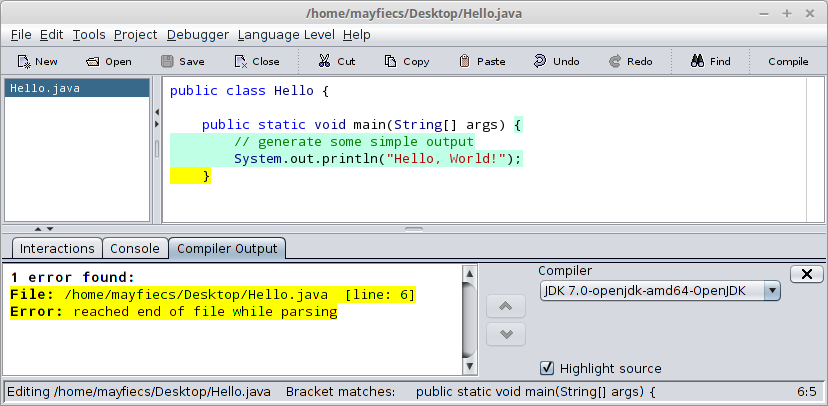
\includegraphics[width=\textwidth]{syntax-error.png}
\caption{A syntax error caused by a missing brace.}
\end{figure}

To make matters worse, the error messages you get from the compiler are often not very helpful.
For example, removing the closing brace on line 8 of the hello world program results in ``Error: reached end of file while parsing.''
The compiler also reports that the problem was found on line 6, which in this case is not at fault.
Since line 8 was deleted, the compiler had no other choice.

During the first few weeks of your programming career, you will probably spend a lot of time tracking down syntax errors.
But as you gain experience, you will make fewer errors and find them more quickly.

\subsection{Runtime errors}

\index{runtime error}
\index{error!runtime}
\index{type-safe}
\index{language!type-safe}

The second type of error is a runtime error, so called because it does not appear until after the program has started running.
In Java, these errors occur when the interpreter is executing the byte code and something goes wrong.
Java is designed to be a {\bf type-safe} language, which means that the compiler can detect many potential errors cased by common programming mistakes.
Runtime errors are rare in the simple programs you will see in the first few chapters, so it might be a while before you encounter them.

\index{exception}

These errors are also called {\bf exceptions} because they usually indicate that something exceptional (and bad) has happened.
In most environments they appear as windows or dialog boxes that contain information about what happened and what the program was doing when it happened.
For example, if you accidentally divide by zero you will get an \java{ArithmeticException}:

\begin{small}
\begin{stdout}
Exception in thread "main" java.lang.ArithmeticException: / by zero
    at Hello.main(Hello.java:5)
\end{stdout}
\end{small}

This information is useful for debugging.
The first line gives a brief description of the error (/ by zero).
The subsequent lines report the class and method names (Hello.main), along with the file names and line numbers of where the error occurred (Hello.java:5).
Keep in mind that the exact line where the program crashed may not be the line that needs to be fixed.

\subsection{Semantic errors}

\index{logic error}
\index{error!logic}

The third type of error is the semantic or {\bf logic error}.
If there is an error in your program's logic, it will compile and run successfully in the sense that the computer will not generate any error messages.
But it will not do the right thing.
It will do something else.
Specifically, it will do what you told it to do.
Here is an example of a semantic error in the hello world program:

\begin{code}
public class Hello {

    public static void main(String[] args) {
        System.out.println("Goodbye, world.");
    }

}
\end{code}

Note that this program compiles and runs just fine.
The problem is that the main method is not the program we intended.
The meaning of the program (its semantics) is wrong, because it says goodbye instead of hello.
In addition, world is not capitalized, and it ends with a period instead of an exclamation point.
Identifying semantic errors can be tricky because it requires you to challenge your assumptions about the code.
You will need to work backward by looking at the output of the program, and try to figure out what it is doing.
